\documentclass[aspectratio=169]{beamer}

\usetheme{Madrid}
\usecolortheme{default}
\setbeamertemplate{navigation symbols}{}

\usepackage[utf8]{inputenc}
\usepackage[T1]{fontenc}
\usepackage{lmodern}
\usepackage{booktabs}
\usepackage{amsmath}
\usepackage{array}
\usepackage{sansmath}
\usepackage{tikz}
\usetikzlibrary{arrows.meta, positioning, fit, backgrounds, calc}

\title{PAL: Playtime-aware Attentive Learning\\for Steam Bundle Recommendation}
\subtitle{Framework and Key Innovations}
\author{BT4222 Project Presentation\\Group 13}
\date{\today}

\definecolor{palblue}{RGB}{38,84,124}
\definecolor{palbluefill}{RGB}{232,241,248}
\definecolor{palgreen}{RGB}{66,126,90}
\definecolor{palgreenfill}{RGB}{233,244,236}
\definecolor{palorange}{RGB}{198,114,46}
\definecolor{palorangefill}{RGB}{252,239,229}
\definecolor{palgray}{RGB}{92,92,92}
\definecolor{palink}{RGB}{34,34,34}

\tikzset{
  block/.style={
    draw=palblue,
    rounded corners=2mm,
     very thick,
    fill=palbluefill,
    align=center,
    minimum height=0.95cm,
    text width=2.15cm,
    inner sep=5pt,
    font=\small\sffamily,
    text=palink
  },
  smallblock/.style={
    draw=palgreen!70!black,
    rounded corners=2mm,
    thick,
    fill=palgreenfill,
    align=center,
    minimum height=0.88cm,
    text width=1.95cm,
    inner sep=4pt,
    font=\small\sffamily,
    text=palink
  },
  scoreblock/.style={
    draw=palorange!85!black,
    rounded corners=2mm,
    thick,
    fill=palorangefill,
    align=center,
    minimum height=0.88cm,
    text width=1.95cm,
    inner sep=4pt,
    font=\small\sffamily,
    text=palink
  },
  arrow/.style={-{Latex[length=2.5mm]}, thick, draw=palgray},
  softbg/.style={rounded corners=3mm, fill=black!3, draw=none}
}

\begin{document}

\begin{frame}
  \titlepage
\end{frame}

\begin{frame}{Problem and Data}
  \begin{columns}[T]
    \begin{column}{0.55\textwidth}
      \begin{itemize}
        \item We study \textbf{Steam bundle recommendation}, not single-game recommendation.
        \item Each candidate is a \textbf{bundle of games}; the model ranks bundles for each user.
        \item PAL uses three sparse relations:
        \begin{itemize}
          \item \textbf{User-Bundle}
          \item \textbf{User-Item}
          \item \textbf{Bundle-Item}
        \end{itemize}
        \item Current main dataset: \textbf{SteamDebug}
        \item Auxiliary experiment dataset: \textbf{SteamAffinity}
      \end{itemize}
    \end{column}
    \begin{column}{0.43\textwidth}
      \begin{block}{Why this task is hard}
        \begin{itemize}
          \item A bundle is a \textbf{set} of items
          \item Users may care about different games inside the same bundle
          \item Item-view and bundle-view may not be equally reliable
        \end{itemize}
      \end{block}
    \end{column}
  \end{columns}
\end{frame}

\begin{frame}{PAL Framework}
  \centering
  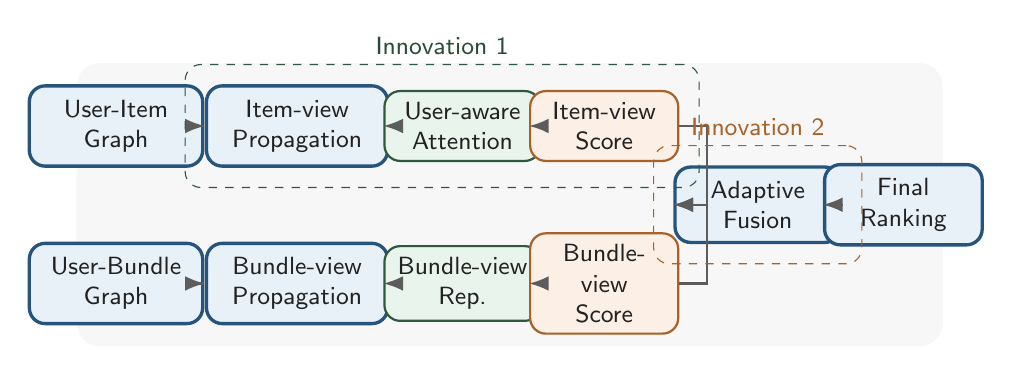
\begin{tikzpicture}[x=1cm,y=1cm]
    \node[softbg, minimum width=11.0cm, minimum height=3.6cm] at (5.0,0) {};
    \node[block, text width=1.85cm] (uib) at (0,1.0) {User-Item\\Graph};
    \node[block, text width=1.85cm] (ubb) at (0,-1.0) {User-Bundle\\Graph};
    \node[block, text width=1.95cm] (itemprop) at (2.3,1.0) {Item-view\\Propagation};
    \node[block, text width=1.95cm] (bundleprop) at (2.3,-1.0) {Bundle-view\\Propagation};
    \node[smallblock, text width=1.7cm] (attn) at (4.4,1.0) {User-aware\\Attention};
    \node[smallblock, text width=1.7cm] (bundlerep) at (4.4,-1.0) {Bundle-view\\Rep.};
    \node[scoreblock, text width=1.6cm] (itemscore) at (6.2,1.0) {Item-view\\Score};
    \node[scoreblock, text width=1.6cm] (bundlescore) at (6.2,-1.0) {Bundle-view\\Score};
    \node[block, text width=1.75cm] (fusion) at (8.15,0) {Adaptive\\Fusion};
    \node[block, text width=1.65cm] (rank) at (10.0,0) {Final\\Ranking};

    \draw[arrow] (uib) -- (itemprop);
    \draw[arrow] (ubb) -- (bundleprop);
    \draw[arrow] (itemprop) -- (attn);
    \draw[arrow] (attn) -- (itemscore);
    \draw[arrow] (bundleprop) -- (bundlerep);
    \draw[arrow] (bundlerep) -- (bundlescore);
    \draw[arrow] (itemscore.east) -- ++(0.35,0) |- (fusion.west);
    \draw[arrow] (bundlescore.east) -- ++(0.35,0) |- (fusion.west);
    \draw[arrow] (fusion) -- (rank);

    \node[draw=palgreen!70!black, dashed, rounded corners=2mm, inner sep=2.5mm, fit=(itemprop)(attn)(itemscore), label={[palgreen!60!black,font=\small\sffamily]above:Innovation 1}] {};
    \node[draw=palorange!85!black, dashed, rounded corners=2mm, inner sep=2.5mm, fit=(fusion), label={[palorange!85!black,font=\small\sffamily]above:Innovation 2}] {};
  \end{tikzpicture}

  \vspace{0.6em}
  \begin{itemize}
    \item Baseline backbone: dual-view graph recommendation
    \item PAL changes \textbf{how bundles are represented} and \textbf{how both views are fused}
  \end{itemize}
\end{frame}

\begin{frame}{Innovation 1: User-aware Item Attention}
  \centering
  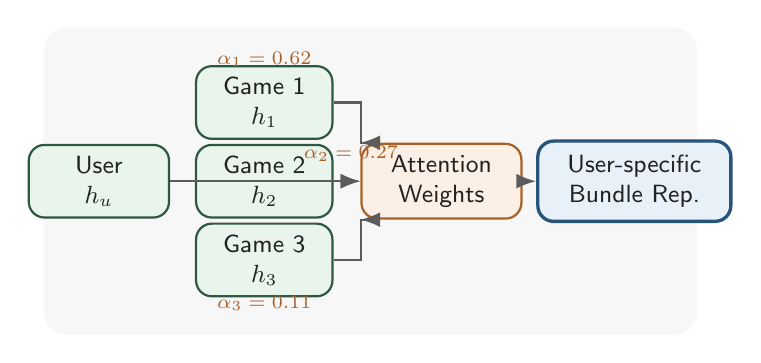
\begin{tikzpicture}[x=1cm,y=1cm]
    \node[softbg, minimum width=8.3cm, minimum height=3.9cm] at (3.45,0) {};
    \node[smallblock, text width=1.5cm] (user) at (0,0) {User\\$h_u$};
    \node[smallblock, text width=1.45cm] (i1) at (2.1,1.0) {Game 1\\$h_1$};
    \node[smallblock, text width=1.45cm] (i2) at (2.1,0) {Game 2\\$h_2$};
    \node[smallblock, text width=1.45cm] (i3) at (2.1,-1.0) {Game 3\\$h_3$};
    \node[scoreblock, text width=1.75cm] (score) at (4.35,0) {Attention\\Weights};
    \node[block, text width=2.1cm] (agg) at (6.8,0) {User-specific\\Bundle Rep.};

    \draw[arrow] (user.east) -- (score.west);
    \draw[arrow] (i1.east) -- ++(0.35,0) |- (score.north west);
    \draw[arrow] (i2.east) -- (score.west);
    \draw[arrow] (i3.east) -- ++(0.35,0) |- (score.south west);
    \draw[arrow] (score) -- (agg);

    \node[text=palorange!85!black, font=\scriptsize\sffamily] at (2.1,1.55) {$\alpha_1=0.62$};
    \node[text=palorange!85!black, font=\scriptsize\sffamily] at (3.2,0.35) {$\alpha_2=0.27$};
    \node[text=palorange!85!black, font=\scriptsize\sffamily] at (2.1,-1.55) {$\alpha_3=0.11$};
  \end{tikzpicture}

  \vspace{0.7em}
  \begin{itemize}
    \item Baseline uses near-fixed item aggregation, so the same bundle looks similar across users.
    \item PAL makes bundle representation \textbf{user-dependent}: different users can focus on different games.
    \item This also gives a direct explanation of \textbf{which items mattered most}.
  \end{itemize}

  \[
    h_b^{I,u} = \sum_i \alpha(u,b,i) h_i
  \]
\end{frame}

\begin{frame}{Innovation 2: Adaptive Cross-view Fusion}
  \begin{columns}[T]
    \begin{column}{0.53\textwidth}
      \centering
      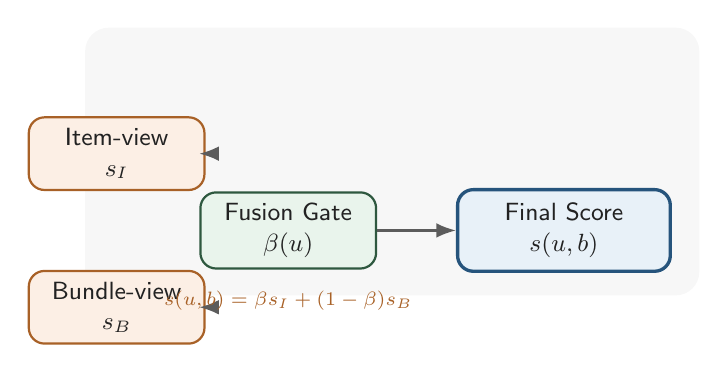
\begin{tikzpicture}[node distance=0.5cm and 0.65cm]
        \node[softbg, minimum width=7.8cm, minimum height=3.4cm] at (3.5,-0.1) {};
        \node[scoreblock] (si) {Item-view\\$s_I$};
        \node[scoreblock, below=1.0cm of si] (sb) {Bundle-view\\$s_B$};
        \node[smallblock, right=1.05cm of $(si)!0.5!(sb)$] (beta) {Fusion Gate\\$\beta(u)$};
        \node[block, right=1.0cm of beta, text width=2.35cm] (final) {Final Score\\$s(u,b)$};

        \draw[arrow] (si.east) -- (beta.west |- si.east);
        \draw[arrow] (sb.east) -- (beta.west |- sb.east);
        \draw[arrow] (beta) -- (final);

        \node[below=0.15cm of beta, text=palorange!85!black, font=\scriptsize\sffamily, align=center] {$s(u,b)=\beta s_I + (1-\beta)s_B$};
      \end{tikzpicture}
    \end{column}
    \begin{column}{0.45\textwidth}
      \begin{itemize}
        \item Baseline effectively assumes a fixed combination of both views
        \item PAL learns \textbf{how much to trust each view}
        \item Rich item histories may favor item-view
        \item Strong bundle interaction patterns may favor bundle-view
        \item The fusion weight is also interpretable
      \end{itemize}
    \end{column}
  \end{columns}
\end{frame}

\begin{frame}{Training Objective}
  \begin{columns}[T]
    \begin{column}{0.52\textwidth}
      \begin{block}{Loss design}
        \[
          \mathcal{L} = \mathcal{L}_{\mathrm{BPR}} + \lambda \mathcal{L}_{\mathrm{CL}}
        \]
        \begin{itemize}
          \item \textbf{BPR loss}: rank positive bundles above sampled negatives
          \item \textbf{Contrastive loss}: align user and bundle representations across the two views
        \end{itemize}
      \end{block}
    \end{column}
    \begin{column}{0.44\textwidth}
      \begin{block}{Why this matters}
        \begin{itemize}
          \item Keeps item-view and bundle-view complementary
          \item Preserves ranking quality
          \item Avoids learning two fully disconnected views
        \end{itemize}
      \end{block}
    \end{column}
  \end{columns}
\end{frame}

\begin{frame}{Evaluation and Explainability}
  \begin{columns}[T]
    \begin{column}{0.47\textwidth}
      \begin{block}{Evaluation metrics}
        \begin{itemize}
          \item Recall
          \item Precision
          \item NDCG
          \item Hit Rate
          \item MAP
          \item MRR
          \item F1
        \end{itemize}
      \end{block}
    \end{column}
    \begin{column}{0.5\textwidth}
      \begin{block}{Exported explanations}
        For each recommended bundle, PAL can export:
        \begin{itemize}
          \item final score
          \item item-view score
          \item bundle-view score
          \item fusion weight
          \item top attended items in the bundle
        \end{itemize}
      \end{block}
    \end{column}
  \end{columns}
\end{frame}

\begin{frame}{What PAL Adds Beyond the Baseline}
  \centering
  \begin{tabular}{>{\raggedright\arraybackslash}p{0.28\textwidth} >{\raggedright\arraybackslash}p{0.27\textwidth} >{\raggedright\arraybackslash}p{0.31\textwidth}}
    \toprule
    Aspect & Baseline & PAL \\
    \midrule
    Bundle modeling in item-view & Mostly fixed aggregation & User-aware attention \\
    View combination & Fixed / naive combination & Adaptive learnable fusion \\
    Interpretability & Limited & Top items + fusion weight \\
    Experiment tracking & Standard setup & CSV, checkpoints, TensorBoard, wandb \\
    \bottomrule
  \end{tabular}

  \vspace{0.9em}
  \begin{block}{Main message}
    PAL is not just a larger model. It introduces \textbf{task-motivated personalization}
    inside bundles and \textbf{task-motivated adaptive reasoning} across views.
  \end{block}
\end{frame}

\begin{frame}
  \centering
  {\LARGE Thank you}

  \vspace{0.9em}
  {\large Questions and feedback are welcome.}
\end{frame}

\end{document}
